\documentclass[11pt]{book}

\usepackage[authoryear]{natbib}
\usepackage{xcolor}
\usepackage[T1]{fontenc}
\usepackage{fourier}
\usepackage[utf8]{inputenc}
\usepackage[hidelinks]{hyperref}
\usepackage{slashbox}
\usepackage{graphicx}
\usepackage{url}
\usepackage{enumitem}
\usepackage[font=small,labelfont=bf]{caption}
\usepackage{float}
\usepackage{amsmath}
\usepackage{algpseudocode}
\usepackage{algorithm2e}

\newcommand{\todo}[1]{\textcolor{red}{[TODO: #1]}\PackageWarning{TODO:}{#1!}}
\newcommand{\note}[1]{\textcolor{red}{[NOTE: #1]}\PackageWarning{NOTE:}{#1!}}
\newcommand*{\np}{\par\noindent\newline}

\title{Agent Based Models of the Formation of Social Preferences}
\author{S Pardy}
\begin{document}
\begin{titlepage}
	\newcommand{\HRule}{\rule{\linewidth}{0.5mm}} % Defines a new command for horizontal lines, change thickness here
	
	\center % Centre everything on the page
	
	%------------------------------------------------
	%	Headings
	%------------------------------------------------
	
	\textsc{\LARGE Monash University}\\[1.5cm]	
	\textsc{\Large Bachelor of Science (Honours)}\\[0.5cm] % Major heading such as course name
	
	\textsc{\large Computational Science}\\[0.5cm] % Minor heading such as course title
	
	%------------------------------------------------
	%	Title
	%------------------------------------------------
	
	\HRule\\[0.4cm]
	
	{\huge\bfseries Agent Based Models of the Formation of Social Preferences}\\[0.4cm]
	
	\HRule\\[1.5cm]
	
	%------------------------------------------------
	%	Author(s)
	%------------------------------------------------
	
	\begin{minipage}{0.4\textwidth}
		\begin{flushleft}
			\large
			\textit{Author}\\
			Sam \textsc{Pardy}
		\end{flushleft}
	\end{minipage}
	~
	\begin{minipage}{0.4\textwidth}
		\begin{flushright}
			\large 
			\textit{Student ID}\\
		25940783   
		\end{flushright}
	\end{minipage}
	\vfill
	\vfill
	{\large
	\textit{Supervisor}\\
	Dr. Julian \textsc{Garcia}}
	
	%------------------------------------------------
	%	Date
	%------------------------------------------------
	
	\vfill\vfill\vfill % Position the date 3/4 down the remaining page
	
	{\large\today} % Date

	\vfill % Push the date up 1/4 of the remaining page
	
\end{titlepage}
% \hypersetup{colorlinks, citecolor=black, filecolor=black, linkcolor=black urlcolor=black}

% \newpage
% \chapter*{Declaration}
% \chapter*{Abstract}
% \chapter*{Acknowledgment}

\tableofcontents
\newpage
\chapter{Introduction}
\section{Preamble}
\section{Motivation \& Objectives}

\chapter{Literature Review}

\chapter[Theoretical \& Experimental Context]{Limitations of Theory \& The Experimental Framework}

The theoretical and analytical work discussed in the previous chapters suffers from several limitations that affect the generality of the conclusions drawn. 
Chiefly, it is static; the conclusions focus on evolutionary stable strategies as a solution concept.
These conclusions may be meaningful however do not tell us anything about how likely these strategies are to evolve or what circumstances may lead to them evolving.
Further, the work is slightly abstract in that in places it does not detail specific attributes of the model it is working with in favour of broader `catch-all' definitions,
this has made the process of creating simulation-based models of the theory difficult at times.
The experimental framework that we have created as part of \textit{this} research seeks to recreate these models as dynamically-evolving before attempting to recover the results achieved in existing, static work.
\todo{Why static v dynamic important? => eq selection, dynamics, diversity}

\section{Limitations of Theory}
\np The primary source of theoretical work that this research has been on based is that of Alger \& Weibull (\citeyear{alger_generalization_2012}, \citeyear{alger_homo_2013}; henceforth, \textit{AW}).
This work finds that under certain assumptions a utility function that is centred around a linear relationship between the two players' payoffs results in evolutionarily stable play.
This utility function is given in equation \ref{linearESSEquation}, in which \textit{x} and \textit{y} are types in the population and $\alpha$ is equal to the \textit{index of assortativity}.
\begin{equation}
	\label{linearESSEquation}
	u_\alpha(x, y, ) = \Pi(x,y) + \alpha\Pi(y,x)
\end{equation}

\noindent To achieve this, the authors assume that all types have a utility function of the same form as \ref{linearESSEquation} where $\alpha \in (-1, 1)$ \citep[p. ~47]{alger_generalization_2012}.
With this assumption, the model, in essence, only allows one number ($\alpha$) to freely evolve.
This assumption severely limits the search space of the evolutionary process. 
The experimental framework that we have created relaxes this assumption.

\np A further assumption made in AW is that while players do not have information about their opponent's preferences,
the players converge to "mutually compatible" strategies and, in effect, play a Nash equilibrium with perfect information \citep[p. ~46]{alger_generalization_2012}.
It is unclear how realistic this assumption is. 
As discussed in previous chapters, it does not make sense to assume that players have knowledge about their opponent's preferences 
but it may be acceptable to assume that when engaging in repeated interactions players converge to Nash equilibrium play relatively quickly.
It is possible, though, that this assumption impacts the evolutionarily process substantially. 
Our experimental framework relies on this assumption also.

\np Commonly in the literature it is assumed that the agents will be matched to play symmetric, two-player games.
This is true also of \citet{alger_generalization_2012}.
In general, a \textit{symmetric} two-player game entails that an agent is indifferent (in terms of payoffs) as to which of the players she takes the roles of in the interaction.
This assumption makes easier our job of implementing a fitness-comparison mechanism.
As fitness is linked to the respective payoff achieved by each agent, the fact that the net payoff on offer to each player is equal simplifies the eventual fitness comparison.
However, we will see later that this assumption may have contributed to some bias in the sampling.

\np A final assumption to note is that the fitness used in the model in \citet{alger_generalization_2012} is that of \textit{average} fitness.
This measure is less stringent than measures used elsewhere (notably in \citet{alger_homo_2013}). 
An oft used fitness measure requires that for an invasion to occur, a mutant must achieve a higher payoff in all equilibria of all games the two types play when they're matched.

\np Of course, these assumptions are all made within the context of a model that is static.
The conclusions drawn in the work referenced above tend to be of the form \textit{should} a utility function of the form \textit{x} evolve it will result in evolutionary stable play given the assumptions.
The experimental framework we create intends to investigate these conclusions and assumptions in a dynamically evolving environment.
\todo{emphasise how big an asusmption static is}



\section{The Experimental Framework}
A large part of the work undertaken in support of this research involved the creation of an experimental framework that could be used to attempt to recover the results of \citet{alger_generalization_2012} in a dynamically evolving environment.
At a high level this experimental framework is simple, however when digging into the detail, complications arise.
Fundamentally, the framework is made up of a representation of a utility function, 
a means by which instances of this representation can be mutated and a means by which the fitness of two different utility functions can be compared.
With these building blocks we can construct the main loop of the experiments that are undertaken.
We define some utility function that represents our initial resident agent, the resident is then mutated (creating the mutant). 
The fitnesses of both resident and mutant are then computed and compared. 
If the mutant achieves a higher payoff an invasion occurs: the original resident is discarded and the mutant takes over as the new resident.
This process is repeated for a given number of generations.
In the following, we discuss the implementation detail of each of these fundamental parts of the framework, beginning with fitness.


\paragraph{Fitness}
\np Decisions we make about how we measure fitness and what difference in fitness is enough to trigger an invasion can have significant impact on the dynamics of the system.
This is an area in which Alger \& Weibull give us limited but essentially sufficient guidance.
Fitness is measured as the \textit{personal payoff} earned by each type when both players act in accordance with their own preferences.
For an individual $\theta$ in a population state $(\theta, \theta', \epsilon,\sigma)$,
where $\theta'$ is the mutant, $\epsilon$ is the mutant share of the population and $\sigma$ is the \textit{index of assortativity}, the expected fitness gain of the resident and mutant after one interaction is given by equations \ref{FexpectedPayoff} \& \ref{GexpectedPayoff} respectively.
Where $f(x, y)$ is the expected payoff earned by $x$ when facing $y$ in a given interaction.
\newline
\begin{gather}
	\label{FexpectedPayoff}
	F_{\epsilon, \sigma}(\theta, \theta') = (\sigma +(1-\epsilon)(1-\sigma))f(\theta, \theta) + \epsilon(1-\sigma)f(\theta, \theta')\\
	\label{GexpectedPayoff}
	G_{\epsilon, \sigma}(\theta', \theta) = (\sigma +\epsilon(1-\sigma))f(\theta', \theta') + (1-\epsilon)(1-\sigma)f(\theta', \theta)
\end{gather}

\np The notion of evolutionary stability is defined as follows: for a state to be considered stable, the residents must achieve, \textit{on average}, a fitness at least as high as that achieved by the mutants in a population that contains both resident and mutant types.
Using functions \ref{FexpectedPayoff} and \ref{GexpectedPayoff}, this relation is given by \ref{ESSweakInequality}.
\begin{equation}
	\label{ESSweakInequality}
	F_{\epsilon, \sigma}(\theta, \theta') \geq G_{\epsilon, \sigma}(\theta', \theta)
\end{equation}
\citet[~p. 44]{alger_generalization_2012}
\np So, if inequality \ref{ESSweakInequality} does not hold, an invasion occurs.

\begin{figure}[H]
	\centering
	\begin{algorithm}[H]
		\KwData{$\theta$, $\theta'$}
		\KwResult{fitness of $\theta$}
		thetaFitness = 0\;
		\For{specified number of games}{
		 randomly sample payoffs to create new \textit{payoffGame}\;
		 transform \textit{payoffGame} using both individual's utility functions to create \textit{utilityGame}\;
		 \For{each equilibrium in utilityGame}{
		  increase \textit{thetaFitness} by the expected payoff of playing \textit{equilibrium} in \textit{payoffGame}\;
		 }	   
		}
		return (thetaFitness $\div$ number of equilbria in \textit{utilityGame}s)\;
	   \end{algorithm}
	\caption{Pseudocode for the algorithm to perform a fitness comparison.}
	\label{psuedocodeForf}
\end{figure}

\np The place where we are left to make some of our own decisions regarding fitness is in deciding what constitutes the expected payoff function, $f(x,y)$.
Since the authors assume that an \textit{average} payoff is used, the expected payoff function is implemented as the average expected payoff across all equilibria, across all games that individuals play in a given interaction.
Figure \ref{psuedocodeForf} shows a pseudocode for the function $f$.

\np This discussion of expected payoff raises the question of the kinds of games that will be played in these interactions - this is the topic of our next discussion.

\begin{figure}[H]
	\vspace{30px}
	\centering
	\begin{tabular}{|l||*{5}{c|}}\hline
		\backslashbox{Player A}{Player B}
		&\makebox[7em]{Action 1}&\makebox[7em]{Action 2}\\\hline\hline
		Action 1 & a, a & b, c\\\hline
		Action 2 & c, b & d, d \\\hline
	\end{tabular}
	\caption{Payoff matrix detailing the payoff structure of a symmetric game. Where Player A earns the payoff on the left of the cell, and Player B the payoff on the right, and ${a, b, c, d} \in R$.}
	\label{symmetricGame}
	\vspace{20px}
\end{figure}
\paragraph{Games}
\np A key part of any game-theoretic model that attempts to represent the process of preference formation, is the kinds of games that are played.
For the most part, the literature (\citet{alger_generalization_2012}, \citet{alger_homo_2013}, \citet{newton_preferences_2017}) is largely agnostic about the games that are played in the models the work describes.
This work assumes only that the games are symmetric and two player. 
With this assumption in mind, \ref{symmetricGame} shows the payoff structure of a symmetric game.

\np Given that we are interested in how cooperative preferences can develop, we begin with a model in which individuals are matched to play a single type of non-cooperative game.
For example, using a prisoner's dilemma type we can write down a game with the payoff structure detailed in figure \ref{symmetricGame} with payoffs $c > a > d > b$.
Next, we investigate how preferences form when individuals play many different symmetric games in one interaction.
Now, the payoffs $a$ through $d$ are determined as follows:
\begin{center}
	
$a \sim U(0,\phi) \qquad a \in I$

$b \sim U(0,\phi) \qquad b \in I$

$c \sim U(0,\phi) \qquad c \in I$

$d \sim U(0,\phi) \qquad d \in I$
\end{center}

\np In other words, $a, b, c, d$ are independent and identically distributed uniform random variables from $0$ to some maximum $\phi$.

\np \todo{Might say something about asymmetric games here}

\np In Chapter \ref{results_discussion} we discuss results relating to both single- and many-game interactions.


\paragraph{Representing \& Mutating Individuals}
\np The way that utility function types are mutated is intrinsically tied to way that those types are represented in the framework, so we will here discuss them together.
Fundamentally, a utility function in this context is a way to convert the outcomes experienced by two individuals into the utility of one of those individuals.
The individual then acts so as to maximize their utility, and in this way acts like an individual who \textit{prefers} strategy $x$ to strategy $x'$ \textit{iff} $u(x, y) > u(x', y)$.
The experimental framework we setup maintain two ways in which individuals can be represented.
The first method involves maintaining a `utility surface' directly. 
So, an individual is represented as a matrix of utility values that can be queried by payoff.
Mutation is performed by making small, localised changes to an area of the surface.
The second style of representation involves maintaining a two parameter function $f(x,y)$, where x is the payoff earned by the agent whose utility function $f$ is and y is the payoff earned by their opponent. 
Mutation is performed via symbolic regression leaning heavily on the work of \citet{fenton_ponyge2:_2017}.
Both of these representations will be discussed in detail in the following chapter.


\chapter{Results \& Discussion}\label{results_discussion}

\paragraph{Games matter}
		
> Must sample many different kinds of games.
\np When running simulations in which each type's fitness is determined by their expected payoff when playing the above game,
it becomes clear that only mutations that occur near to the payoff points ever lead to invasions. 
The payoff points are the four potential outcomes (in terms of payoffs for each player) of the game: (3,3), (0,4), (4, 0) \& (1, 1).
Plotted in figure \ref{prisoners_payoff_plot}.
\begin{figure}
	\centering
	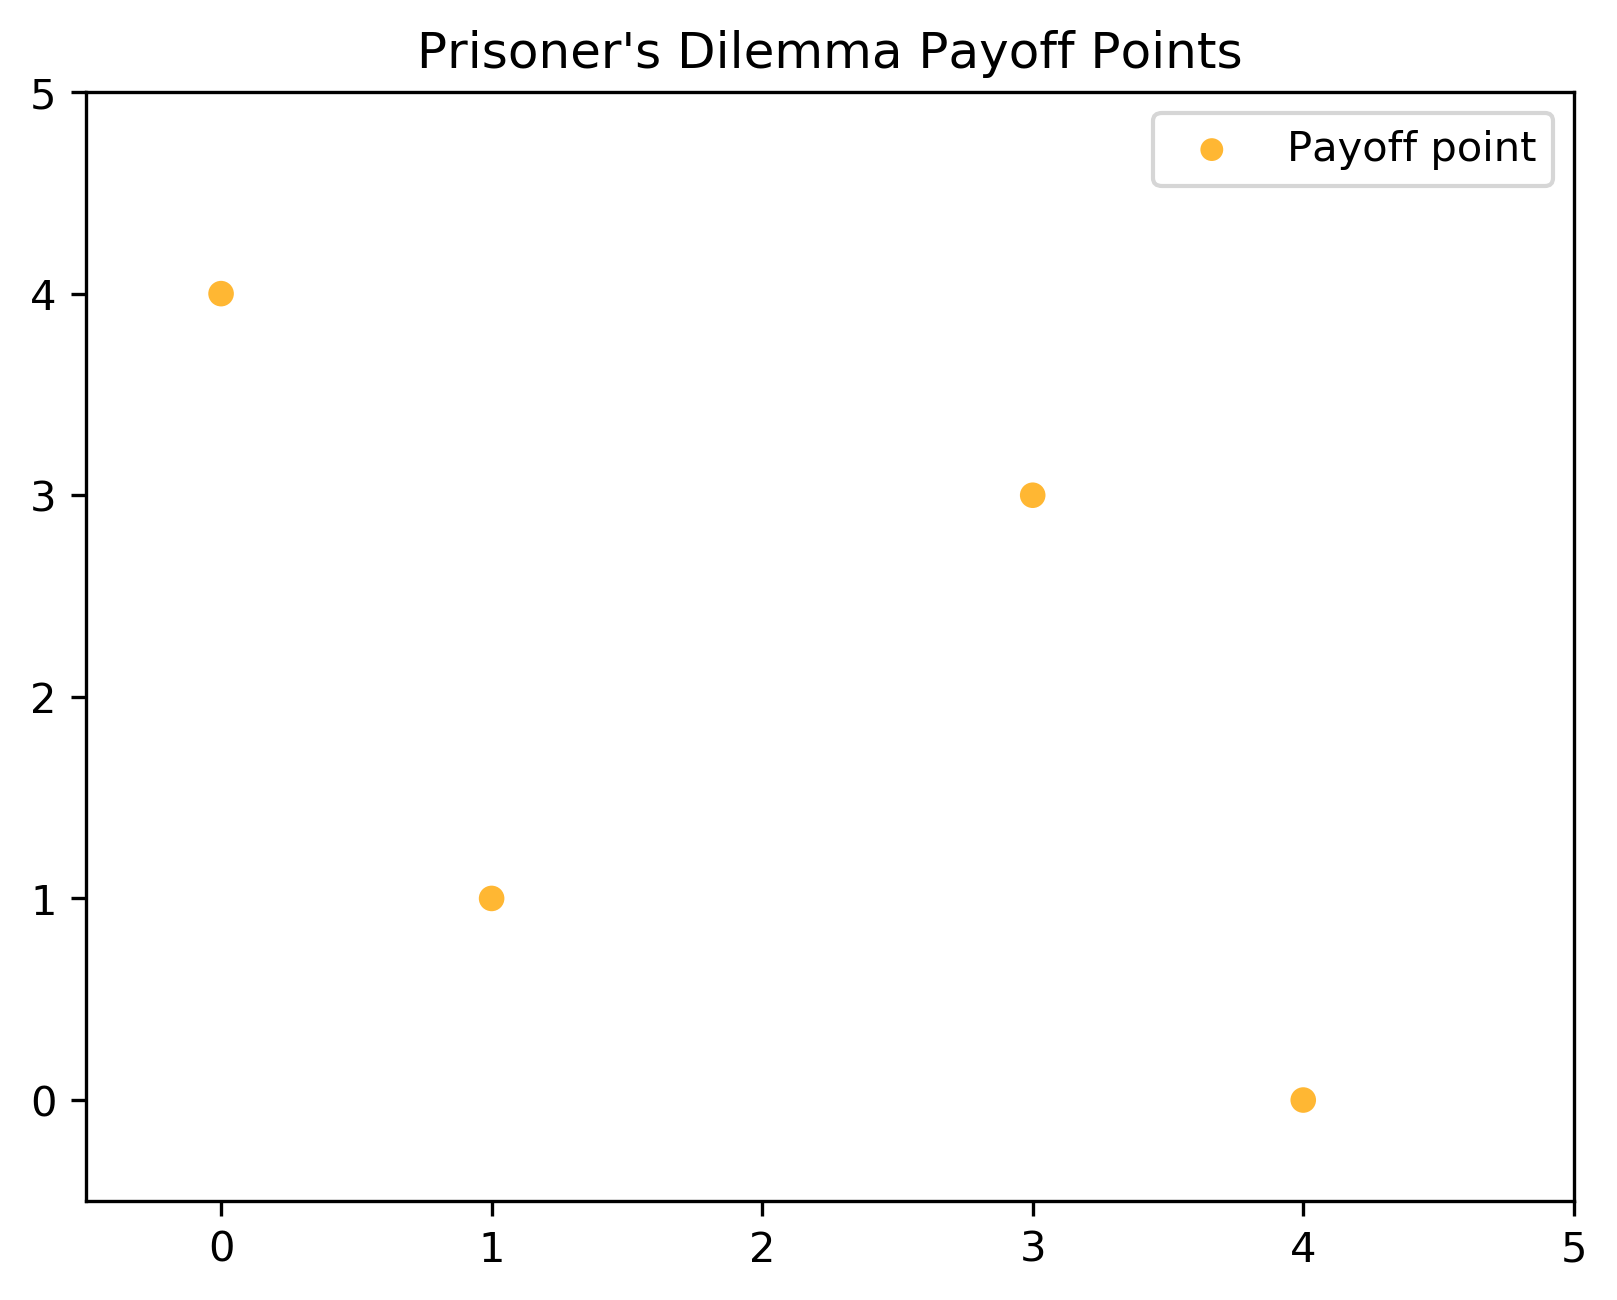
\includegraphics[scale=0.75]{resources/prisoners_dilemma_payoffs.png}
	\caption{The payoff points in a prisoner's dilemma game.}
	\label{prisoners_payoff_plot}
\end{figure}

\np The fact that limited invasions occur in this scenario makes sense when several facts about the model are considered:
\begin{enumerate}[label=(\alph*)]
	\item mutations can occur anywhere within the space and are small.
	\item the fitness of the agents (resident and mutant) is equal in areas of the surface not affected by the mutation.
	\item for a mutant to invade, they must achieve a fitness \textit{greater} than that achieved by the resident - as opposed to greater than or equal to.	
\end{enumerate} 
\np
So, if a mutation occurs at the point (2, 2), given that this mutation has a relatively small radius, 
the expected payoff of the mutant will not differ from that of the resident because the mutation does not touch any of the payoff points.
Hence, the fitnesses are equal, and no invasion occurs. Running large scale simulations using this model results in `utility surfaces' like figure \todo{prisoner's dillema run}.

> JTB result is strongly dependent on the assumption of symmetric games.

\noindent> Phenotypic mutation takes ages.

\noindent> Successful symbolic regression results are strongly dependent on un-biased (or maybe `biased in the right way') grammars.


\section{Phenotypic Mutation}
The first technique of representing utility functions we'll discuss we've called `phenotype mutation'.
This is because in this method individuals are represented directly as a surface in 3 dimensions.
So the only information maintained about different types is their phenotype and mutation is performed directly on the phenotype.
Those dimensions being: my payoff, my opponent's payoff, and my utility.
Figure \ref{selfishUtilitySurface} is an example of a purely selfish utility surface.

\begin{figure}
	\centering
	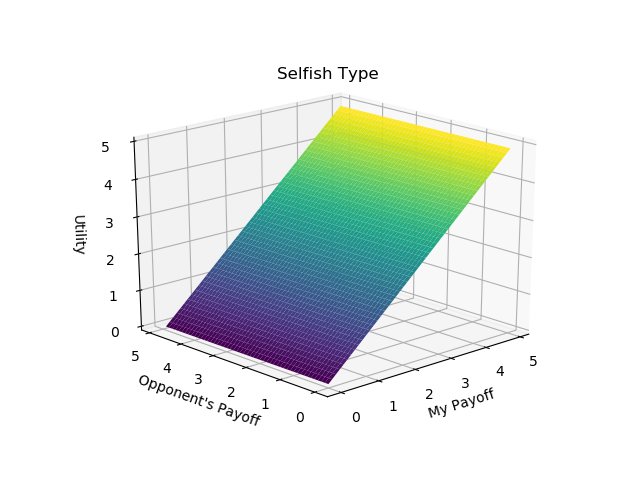
\includegraphics[scale=0.75]{resources/selfish.png}
	\caption{An example of a purely selfish type represented as a `utility surface'.}
	\label{selfishUtilitySurface}
\end{figure}


\np This method has two immediate limitations. 
The first is that the matrix is only defined for a certain payoff range and so a value, $\phi$ must be provided that represents the maximum \textit{payoff} achievable by either individual.
Second, the matrix is discrete and so is accurate only up to a certain granularity - a value, $s$ must be provided that is the `step' of the grid.
The value $s$ should be as small as is computationally feasible. 
Figure \ref{selfishUtilityGrid} is an example of the grid values of a utility surface of an individual that is purely selfish.

\begin{figure}
\[
	\begin{bmatrix} 
	0. & 0. & 0. & \dots & 0. & 0. & 0.\\
	0.1 & 0.1 & 0.1 & \dots & 0.1 & 0.1 & 0.1\\
	0.2 & 0.2 & 0.2 & \dots & 0.2 & 0.2 & 0.2\\
	\vdots & \vdots & \vdots & \dots & \vdots &\vdots &\vdots\\
	4.7 & 4.7 & 4.7 & \dots & 4.7 & 4.7 & 4.7\\
	4.8 & 4.8 & 4.8 & \dots & 4.8 & 4.8 & 4.8\\
	4.8 & 4.8 & 4.8 & \dots & 4.8 & 4.8 & 4.8 
	\end{bmatrix}
\]
\caption{A `selfish' utility grid with $\phi = 5$ and $s = 0.1$.}
\label{selfishUtilityGrid}
\end{figure}

\np Phenotypic mutation is undertaken by performing a small perturbation to the resident surface in a randomly selected area.
This perturbation takes the shape of a bivariate normal distribution with some random $\sigma$, $\sigma \leq \gamma$, where $\gamma$ is parameter of the model.
This method ensures that mutations are small.
It also has the effect of creating \textit{localised} mutations: mutations that only affect a certain area of the surface rather than the shape of the surface overall.
It turns out that the localised nature of these mutations is important and will be discussed in proceeding sections. Figure 

\begin{figure}
	\centering
	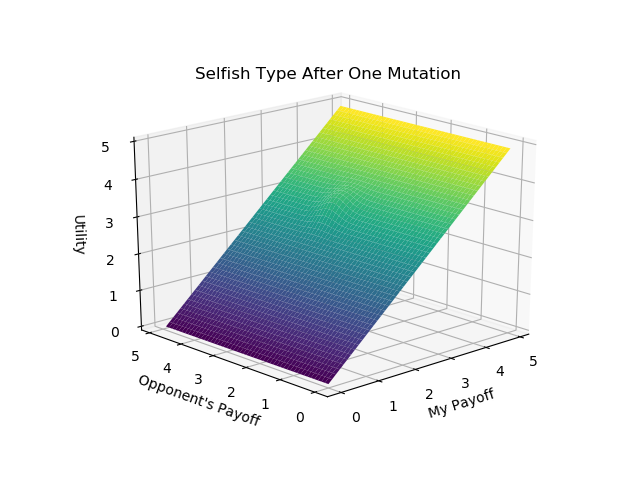
\includegraphics[scale=0.75]{resources/one_mutation.png}
	\caption{The selfish utility surface after one mutation has been applied at the point (3, 3).}
	\label{selfishUtilitySurfaceOneMutation}
\end{figure}


\section{Symbolic Regression}

\chapter{Conclusion}


\todo{is this to speculative/waffley?}
Intuitively, the non-meaningful results achieve when sampling only one kind of game fit with our analogy of the utility function in some way representing the real-world preferences of some agent.\
In reality, agents face many more kinds of situations than just one instance of a prisoner's dilemma,
and so to generate a utility function that is potentially recognisable as one of a real-world agent the function will need to be resilient to many different situations.


\bibliography{thesis}
\bibliographystyle{apalike}

\end{document}